\documentclass[11pt,a4paper]{article}

\onecolumn

\usepackage{ucs}
\usepackage[utf8x]{inputenc}
\usepackage[T1]{fontenc}
\usepackage[ngerman]{babel}
\usepackage{multibib}
\usepackage[hyphens]{url}
\usepackage[hidelinks]{hyperref}
\usepackage{graphicx}
\usepackage{chemfig}
\usepackage{chemnum}
\usepackage{chemmacros}
\usepackage{amsmath}
\usepackage{amssymb}
\usepackage{float}

\usepackage{Seminararbeit-Vorlage/seminararbeit-vorlage}

\usepackage[nottoc,numbib]{tocbibind}

\renewcommand{\listoffigures}{\begingroup
\tocsection
\tocfile{\listfigurename}{lof}
\endgroup}

% Use Helvet font globally
\usepackage{helvet}
\renewcommand{\familydefault}{\sfdefault}

% Set distance between two lines
\usepackage{setspace}
\onehalfspacing

\usepackage{mdwlist}

% Indent the first line of a paragraph
\usepackage{indentfirst}

% Set margins
\usepackage{geometry}
\geometry{verbose,a4paper,tmargin=25mm,bmargin=25mm,lmargin=30mm,rmargin=30mm}

% Stick footnotes to the bottom of the page
\usepackage[bottom]{footmisc}

% Print the page number on the center head
\usepackage{scrpage2}
\clearscrheadfoot
\chead{-\ \pagemark\ -}
\pagestyle{scrheadings}

\addto{\captionsngerman}{\renewcommand{\refname}{Quellenverzeichnis}}
\addto{\captionsngerman}{\renewcommand{\figurename}{Abb.}}
\addto\extrasngerman{\def\figureautorefname{Abb.}}

\newcommand\setpolymerdelim[2]{\def\delimleft{#1}\def\delimright{#2}}
\def\makebraces[#1,#2]#3#4#5{%
\edef\delimhalfdim{\the\dimexpr(#1+#2)/2}%
\edef\delimvshift{\the\dimexpr(#1-#2)/2}%
\chemmove{%
\node[at=(#4),yshift=(\delimvshift)]
{$\left\delimleft\vrule height\delimhalfdim depth\delimhalfdim width0pt\right.$};%
\node[at=(#5),yshift=(\delimvshift)]
{$\left.\vrule height\delimhalfdim depth\delimhalfdim width0pt\right\delimright_{\rlap{$\scriptstyle#3$}}$};}}
\setpolymerdelim[]

% Start document
\begin{document}

% Frontpage
\title{Transparente Kunststoffe in der Informationstechnologie}
\author{Tobias Schmidt}
\school{RUDOLF-DIESEL-GYMNASIUM AUGSBURG}
\year{2014/2016}
\subject{Chemie}
\seminar{Kunststoffchemie}
\supervisor{Fr. Müllerburger}
\deadline{10.11.2015}
\genderAuthor{m}
\genderSupervisor{f}
\maketitle

\thispagestyle{empty}

\tableofcontents

\section{Speicherung und Weitergabe von Informationen im historischen Kontext}

Informationen speichern und weitergeben ist zentraler Bestandteil der
menschlichen Kultur und führte in der Menschheitsgeschichte zu bahnbrechenden
Erfindungen und laufenden Innovationen.

In der Steinzeit wurden Informationen an Höhlenwände gemalt, ab dem 3.
Jahrtausend vor Christus mittels Keilschrift (siehe \autoref{fig:keilschrift})
in Steintafeln gemeißelt und in der Antike auf Papyrus gezeichnet. Mitte des 15.
Jahrhunderts revolutionierte dann Gutenberg die Informationsweitergabe mit der
Erfindung des Buchdrucks, der die Produktion von Büchern in hohen Stückzahlen
und zu geringen Kosten möglich machte. Auch heute noch wird diese Technik für
die Reproduktion von Texten verwendet.

Ende des 19. Jahrhunderts gelang es erstmals, Musik zu speichern. Hierfür wurden
zunächst Schallplatten aus Hartgummi eingesetzt. Dieser wurde um 1900 dann durch
eine Pressmasse abgelöst, die im Wesentlichen aus Schellack\footnote{harzige
Ausscheidung von Lackschildläusen \cite{schellack}} (siehe
\autoref{fig:schallplatte-schellack}) bestand. Auf 12 Zoll-Schellackplatten
konnten Musikstücke mit ca. 4 Minuten Spielzeit pro Seite gespeichert werden.
Mit dem Einsatz des Kunststoffes Polyvinylchlorid ab den 50er Jahren des 20.
Jahrhunderts verbesserte sich die Tonqualität von Schallplatten deutlich.
Außerdem konnte längere Stücke gespeichert und wiedergegeben werden.
\cite{schallplatte1}

Mit der Compact Cassette (CC, siehe \autoref{fig:compact-cassette}), die 1963
auf den Markt kam, war es dann jedermann möglich, selbst Musik aufzunehmen und
dauerhaft zu speichern \cite{kassette1}. Compact Cassetten verwenden ein
Magnetband, das aus einer langen schmalen Kunststofffolie besteht, die mit einem
magnetisierbaren Material beschichtet wurde \cite{kassette2}.

In den 90er Jahren verdrängte  die Compact Disc (CD) innerhalb weniger Jahren
sowohl die Schallplatte als auch die Compact Cassette. Die CD zeichnet sich
durch ihre hohe Speicherkapazität sowie eine geringe Fehlerquote aus und wurde
deshalb zum universellen Speichermedium für Musik, Dokumente, Bilder und Filme.
\cite{cd_durchbruch}

\begin{figure}[h]
  \begin{center}
      \begin{minipage}[t]{0.3\textwidth}
        \begin{center}
            
\includegraphics[height=0.1\textheight]{Bilder/Einleitung/keilschrift.png}
            \caption[Altpersische Keilschrift \newline \url{http://www.faz.net/aktuell/feuilleton/geisteswissenschaften/keilschriften-zehntausend-freunde-mesopotamiens-1657070.html}]{Altpersische Keilschrift}
            \label{fig:keilschrift}
        \end{center}
      \end{minipage}
      \hspace{0.025\textwidth}
      \begin{minipage}[t]{0.3\textwidth}
        \begin{center}
            \includegraphics[height=0.1\textheight]{Bilder/Einleitung/schallplatte-schellack.png}
            \caption[Schellackschallplatte \newline \url{https://de.wikipedia.org/wiki/Datei:Schallplatte_Deutsche_Grammophon_Stimme_seines_Herrn.jpg}]{Schellackschall-platte}
            \label{fig:schallplatte-schellack}
        \end{center}
      \end{minipage}
      \hspace{0.025\textwidth}
      \begin{minipage}[t]{0.3\textwidth}
        \begin{center}
            \includegraphics[height=0.1\textheight]{Bilder/Einleitung/compact-cassette.png}
            \caption[Compact Cassette \newline \url{https://de.wikipedia.org/wiki/Datei:Compactcassette.jpg}]{Compact Cassette}
            \label{fig:compact-cassette}
        \end{center}
      \end{minipage}
  \end{center}
\end{figure}

Kunststoffe sind - wie die oben aufgeführten Beispielen zeigen - für die
Informationstechnologie schon jetzt unersetzbar und kommen - neben der
Speicherung - auch bei der Übertragung großer Datenmengen zum Einsatz.

Sowohl für die Übertragung als auch für das Auslesen von Informationen werden
Lichtsignale verwendet. Hierfür werden vermehrt transparente Materialien
benötigt, die sich für den Alltagsgebrauch eignen.

An den Beispielen der Compact Disc (siehe \autoref{fig:compact-disc}) und der
polymer optischen Faser (POF,  siehe \autoref{fig:pof}) werden in dieser Arbeit
der Einsatz von transparenten Kunststoffen in der Informationstechnologie und
ihre spezielle Eignung behandelt. Dabei wird auf die Funktionsweise und
Produktion von optischen Datenträgern und optischen Wellenleitern eingangen.
Außerdem werden die physikalischen Eigenschaften und die Herstellung der
verwendeten Kunststoffe erläutert.

\begin{figure}[h]
  \begin{center}
      \begin{minipage}[t]{0.3\textwidth}
        \begin{center}
            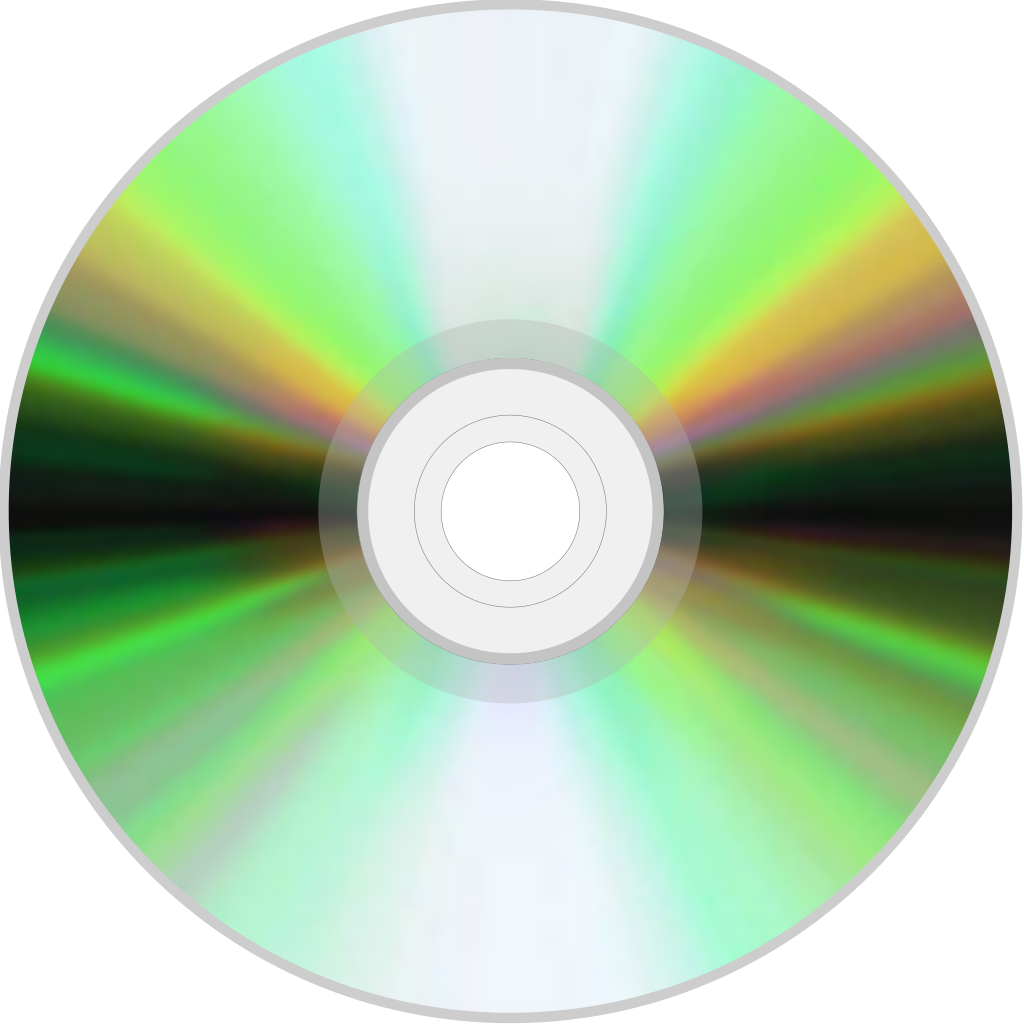
\includegraphics[height=0.1\textheight]{Bilder/Einleitung/compact-disk.png}
            \caption[Compact Disc \newline \url{https://en.wikipedia.org/wiki/File:Compact_disc.svg}]{Compact Disc}
            \label{fig:compact-disc}
        \end{center}
      \end{minipage}
      \hspace{0.025\textwidth}
      \begin{minipage}[t]{0.3\textwidth}
        \begin{center}
            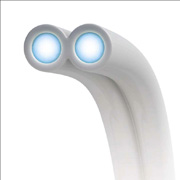
\includegraphics[height=0.1\textheight]{Bilder/Einleitung/pof.png}
            \caption[polymer optischen Faser \newline \url{http://www.heise.de/tr/imgs/08/2/5/4/2/1/5/c337ef89957e0f2b.jpg}]{polymer optischen Faser}
            \label{fig:pof}
        \end{center}
      \end{minipage}
  \end{center}
\end{figure}

\section{Optische Datenträger - die Compact Disc}
\label{sec:cd}

\subsection{Geschichte der Compact Disc}
\label{subsec:cdgeschichte}

Die Entwicklung von optischen Datenträgern für laserbasierte Auslesesysteme
begann in den 70er Jahren des \nolbreaks{20. Jahrhunderts}. 1975 brachte Philips
den ersten optischen Datenträger auf den Markt, die Laservision Videodisc (siehe
\autoref{fig:videodisc}). Sie sollte eine Alternative zum VHS-Videosystem (siehe
\autoref{fig:vhs}) darstellen, war jedoch aufgrund der geringen Verkaufszahlen
nicht erfolgreich.

\ifthenelse{\boolean{showPics}}{
    \begin{figure}[h]
        \begin{center}
            \begin{minipage}[t]{0.4\textwidth}
                \begin{center}
                    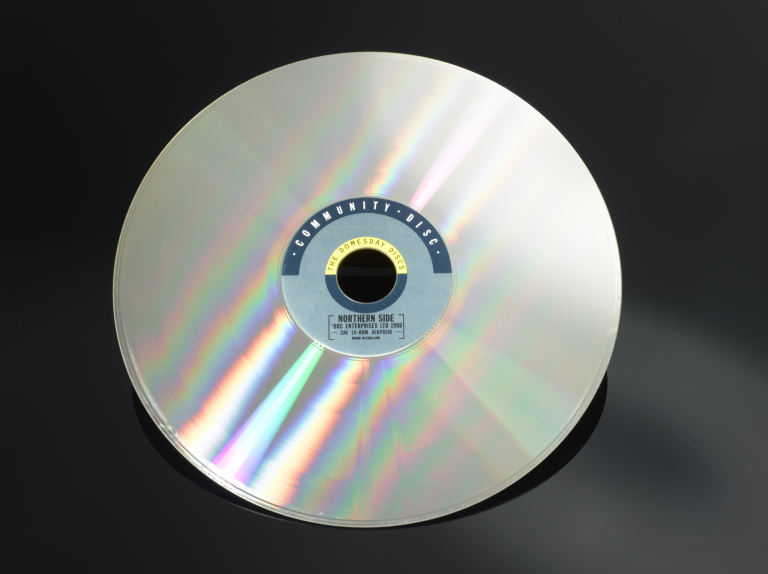
\includegraphics[height=0.1\textheight]{Bilder/Optische_Datentraeger_Die_Compact_Disc/Geschichte/videodisc.png}
                    \caption[Laservision Videodisc \newline \url{http://www.sciencemuseum.org.uk/online_science/explore_our_collections/objects/index/smxg-8095649} (zuletzt aufgerufen am 19.09.2015)]{Laservision Videodisc}
                    \label{fig:videodisc}
                \end{center}
            \end{minipage}
            \hspace{0.025\textwidth}
            \begin{minipage}[t]{0.4\textwidth}
                \begin{center}
                    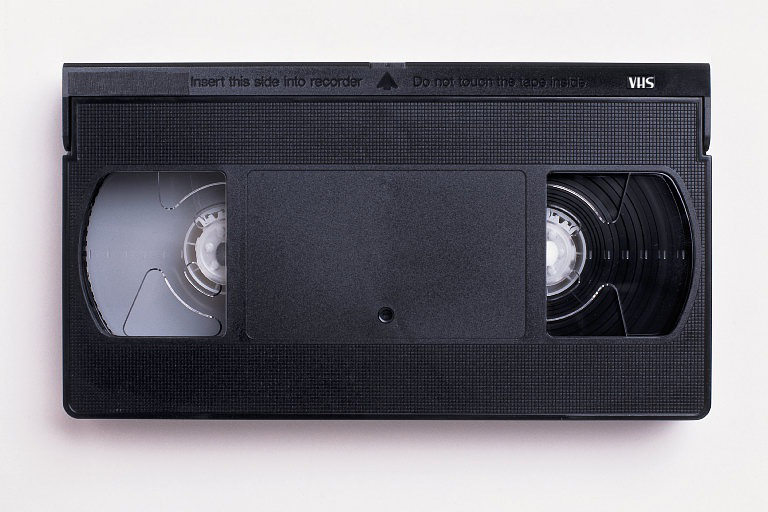
\includegraphics[height=0.1\textheight]{Bilder/Optische_Datentraeger_Die_Compact_Disc/Geschichte/vhs.png}
                    \caption[VHS cassette \newline \url{https://upload.wikimedia.org/wikipedia/commons/6/67/VHS-cassette.jpg} (zuletzt aufgerufen am 19.09.2015)]{VHS Cassette}
                    \label{fig:vhs}
                \end{center}
            \end{minipage}
        \end{center}
    \end{figure}
}{}

Auf Basis der Videodisc entwickelte Philips bis 1977 die Compact Disc Digital
Audio mit einem Durchmesser von \nolbreaks{11,5 cm} und einer Spielzeit von 60
Minuten. Ab 1979 arbeiteten Philips und Sony dann an einem gemeinsamen, noch
heute gültigen CD-Standard mit einem Durchmesser von \nolbreaks{12 cm} und einer
75-minütigen Spielzeit. \cite{cds}

Zunächst scheiterten jedoch die Verhandlungen über Musikrechte für CDs, da die
Schallplattenproduzenten rückläufige Verkaufszahlen befürchteten. Deshalb
konzentrierten sich Philips und Sony auf klassische Musik, da die beiden
Unternehmen zudem annahmen, dass Klassikliebhaber bereit wären, mehr Geld für
eine bessere Klangqualität auszugeben.

Der CD gelang der Durchbruch während der Salzburger Festspiele im Jahr 1981.
Philips und Sony konnten ein Publikum aus Musikkritikern von dem
Zukunftspotential der CD überzeugen. Die Begeisterung der Kritiker erfasste die
internationale Musikszene und bis März 1982 hatten acht Schallplattenfirmen
Verträge mit Philips und Sony unterschrieben. Die Markteinführung erfolgte im
August 1982. \cite{cuz}

Innerhalb weniger Jahre verdrängte die CD die Schallplatte fast komplett vom
Markt. \autoref{fig:umsatzcd} zeigt die Umsatzentwicklung der deutschen
Musikindustrie mit den jeweiligen Tonträgern. Der Umsatz mit Vinylschallplatten,
1980 mit ca. 760 Mio. \euro{} noch das umsatzstärkste Medium, sank bis 1987 erst
all­mäh­lich und dann bis 1992 rapide. Im selben Zeitraum stieg der Umsatz mit
CDs massiv an und erreichte im Jahr 1997 ein Maximum von 2,3 Mrd. \euro{}. Ab
1997 war der Umsatz mit CDs rückläufig, da Privatpersonen selbst CDs \glqq
brennen\grqq{} konnten und zunehmend legale und illegale Angebote im Internet
nutzten.

\ifthenelse{\boolean{showPics}}{
    \begin{figure}[H]
        \begin{center}
            \begin{minipage}[t]{\textwidth}
                \begin{center}
                    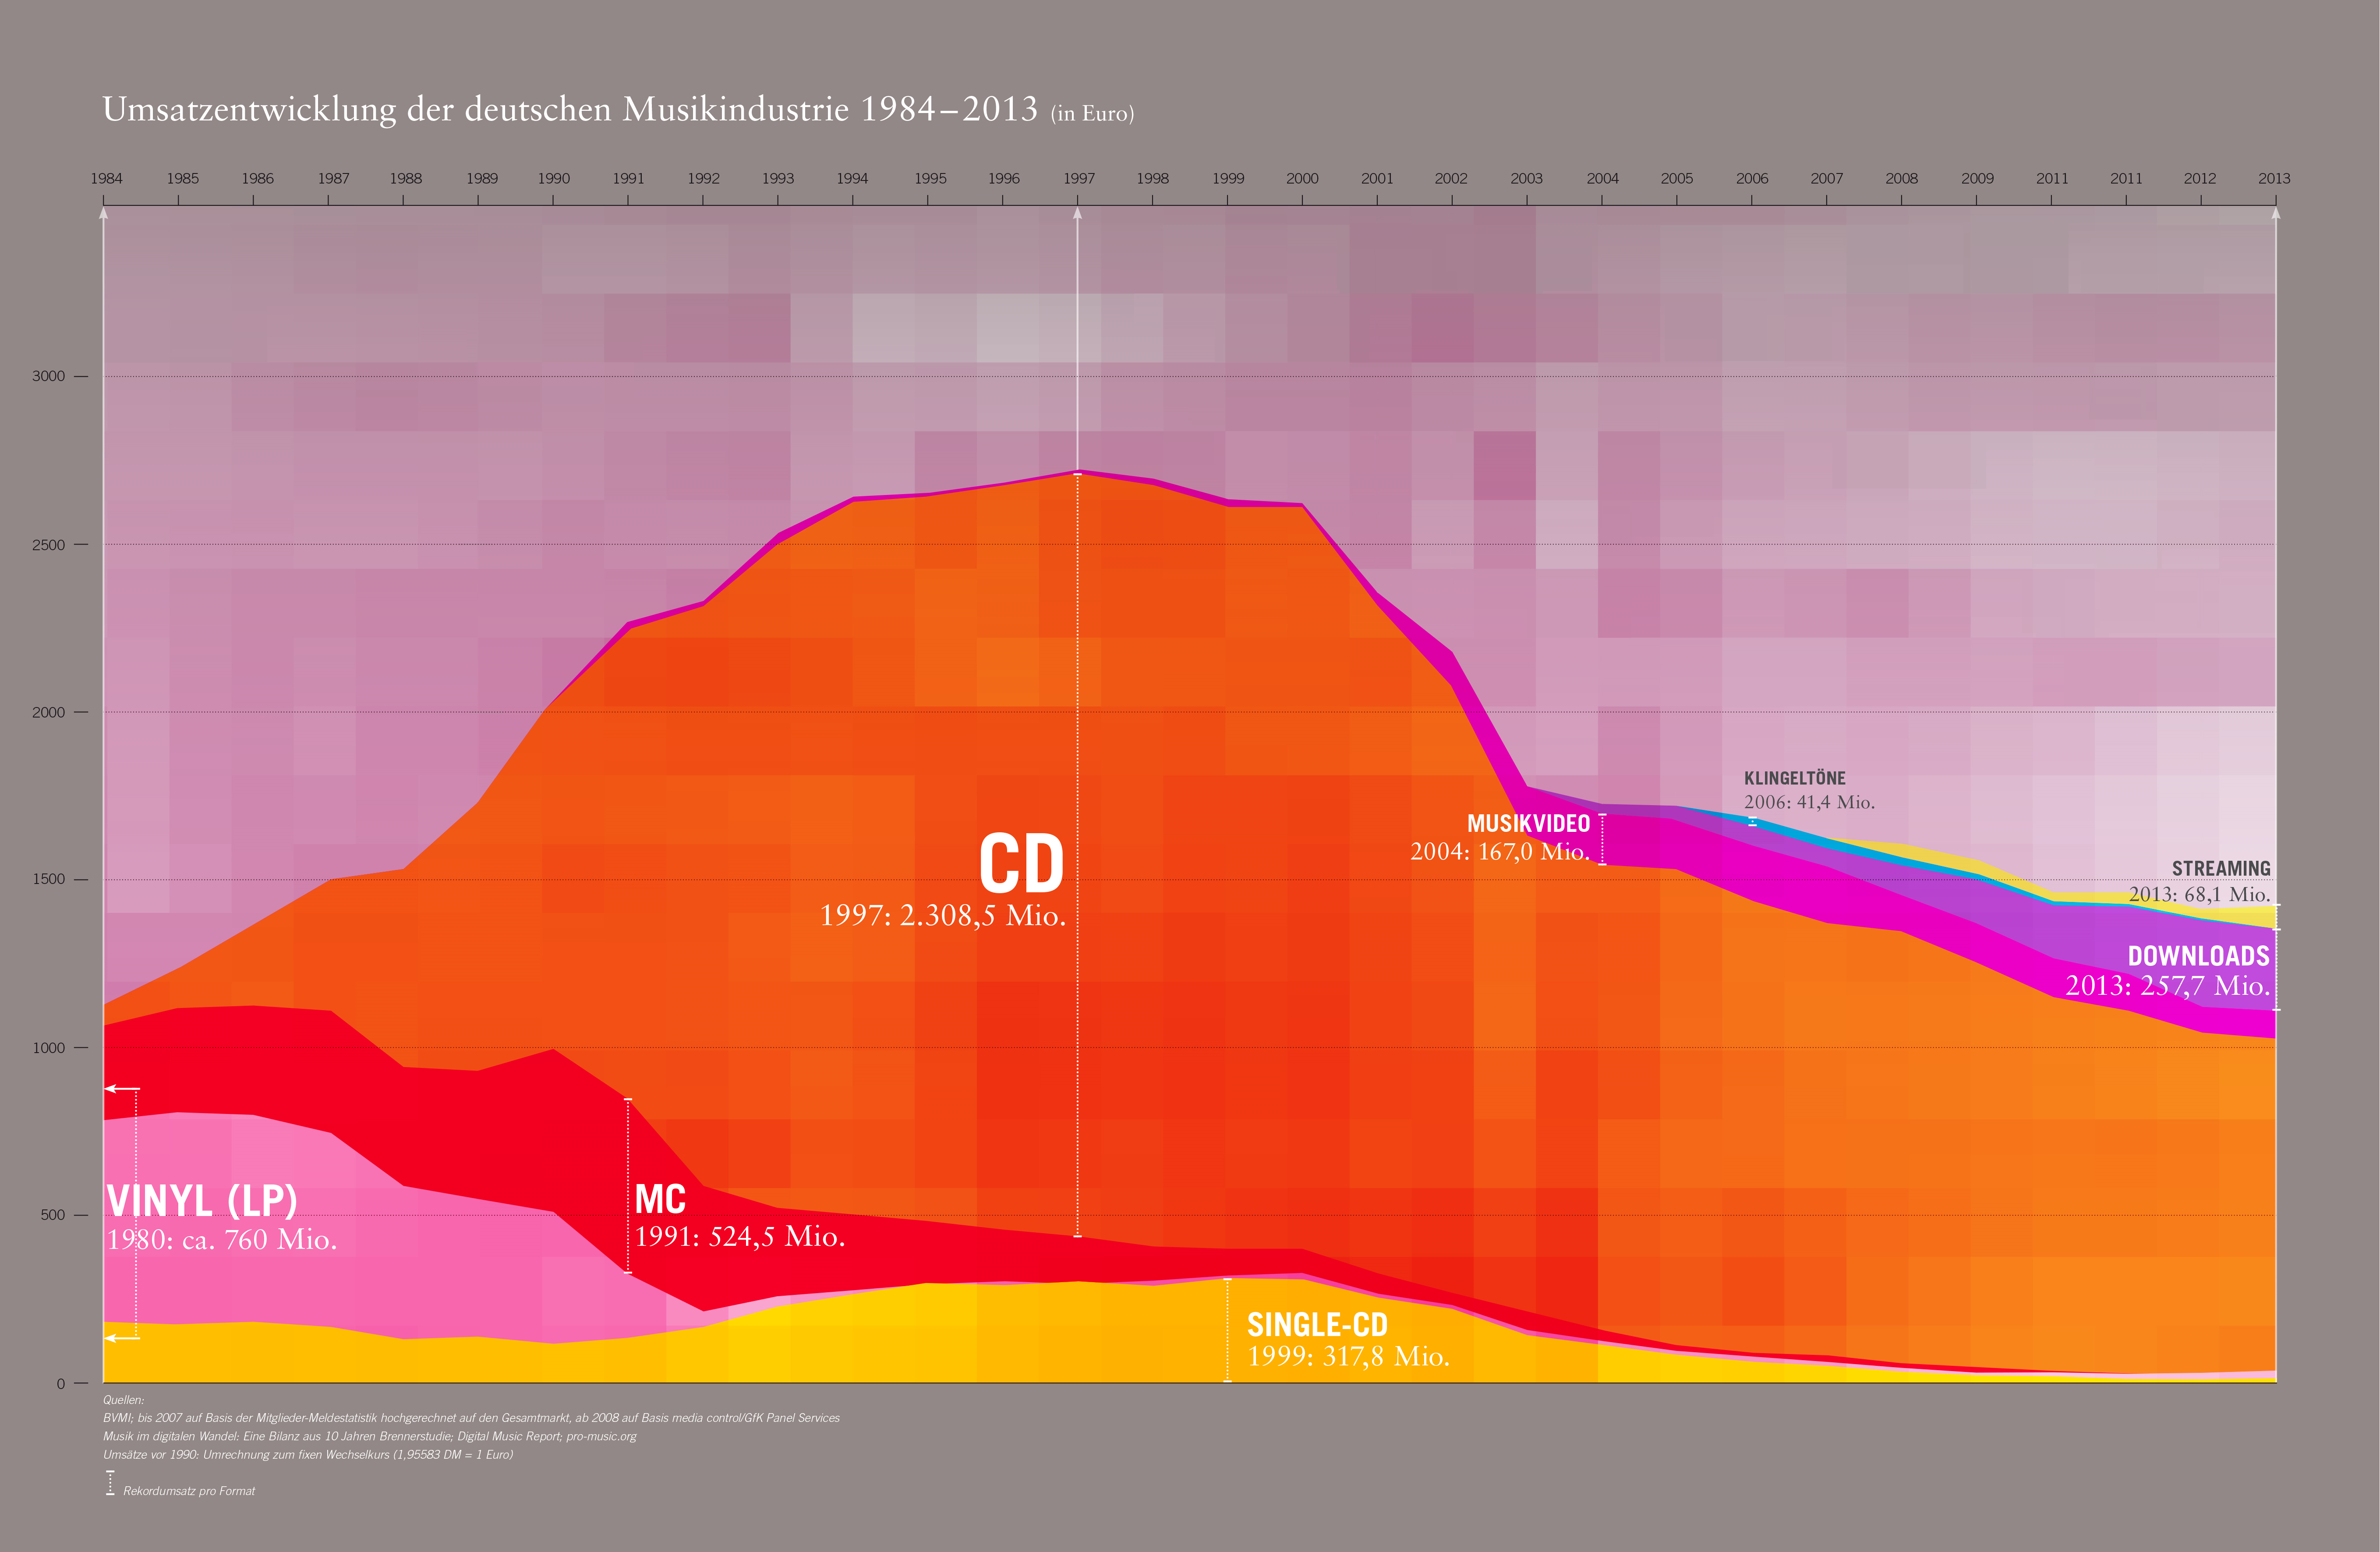
\includegraphics[width=\textwidth]{Bilder/Optische_Datentraeger_Die_Compact_Disc/Geschichte/cdumsatz.png}
                    \caption[Umsatzentwicklung der deutschen Musikindustrie von 1984 bis 2013 \newline verändert nach \url{http://www.musikindustrie.de/uploads/media/140325\_BVMI\_2013\_Jahrbuch\_ePaper\_V02.pdf} S.7 (zuletzt aufgerufen am 03.08.2015)]{Umsatzentwicklung der deutschen Musikindustrie von 1984 bis 2013}
                    \label{fig:umsatzcd}
                \end{center}
            \end{minipage}
        \end{center}
    \end{figure}
}{}

\subsection{Funktionsweise}
\subsection{Herstellung der Compact Disc mittels des Spritzgussverfahrens}
\label{subsec:cdherstellung}

Die Herstellung einer vorbespielten CD beginnt mit der in
\autoref{fig:cdherstellung} dargestellten Anfertigung einer Metallmatrize für
das Spritzgussverfahren. Dafür wird eine Glasplatte mit einem Fotolack
beschichtet und mittels Belichtung wird das \textit{pit}-Muster der CD auf die
Fotolackschicht übertragen. Nachdem der belichtete Fotolack entfernt wurde, kann
ein Negativ der Glasmatrize in Form einer Metallmatrize erstellt werden. Mittels
des Spritzgussverfahrens wird das \textit{pit}-Muster auf eine
Polycarbonatscheibe übertragen. Um eine Reflexionsschicht zu erhalten, wird auf
das Polycarbonat Aluminium aufgedampft. Im letzten Schritt wird die
Reflexionsschicht mithilfe einer Schutzschicht versiegelt. \cite{cdp}

\ifthenelse{\boolean{showPics}}{
    \begin{figure}[h]
        \begin{center}
            \begin{minipage}[t]{\textwidth}
                \begin{center}
                    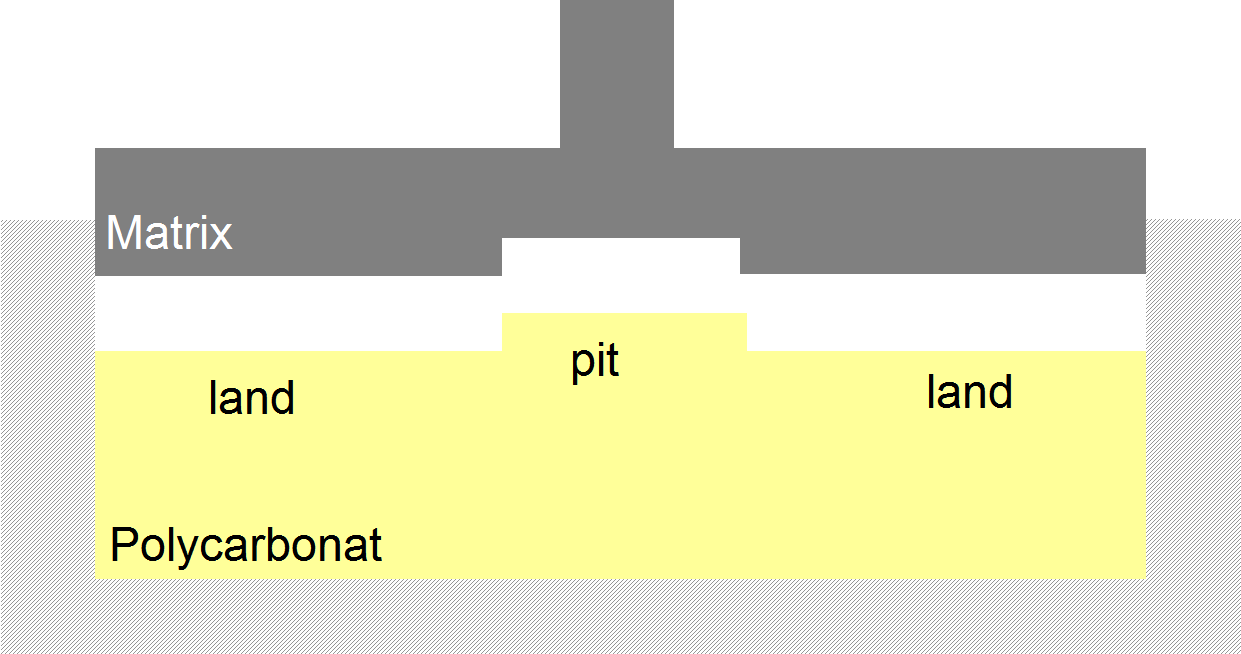
\includegraphics[width=\textwidth]{Bilder/Optische_Datentraeger_Die_Compact_Disc/Herstellung/cdherstellung.png}
                    \caption[Herstellung der Metallmatrize und der CD \newline verändert nach \url{http://www.muenster.de/~asshoff/physik/cd/image46.gif} (zuletzt aufgerufen am 01.11.2015)]{Herstellung der Metallmatrize und der CD}
                    \label{fig:cdherstellung}
                \end{center}
            \end{minipage}
        \end{center}
    \end{figure}
}{}

Das Spritzgussverfahren selbst unterteilt sich in drei Schritte. Wie in
\autoref{fig:cdspritz} zu sehen ist, wird zunächst zerkleinertes Polycarbonat
(Granulat) in die Schnecke eingefüllt. Durch die Heizelemente und die sich
drehende Schnecke verflüssigt sich das Granulat. Dieser Schritt heißt
Plastifizieren. Der sich an der Spitze des Plastifizierzylinders aufbauende
Druck presst die Schnecke teilweise aus dem Zylinder. Danach folgt der
Einspritzvorgang. Dabei wird das geschmolzene Granulat durch die
Vorwärtsbewegung der Schnecke in die CD-Form und auf die Metallmatrize gedrückt.
Nach dem Abkühlen wird die fertige Polycarbonatscheibe ausgeworfen. \cite{cdpf}

\ifthenelse{\boolean{showPics}}{
    \begin{figure}[h]
        \begin{center}
            \begin{minipage}[t]{\textwidth}
                \begin{center}
                    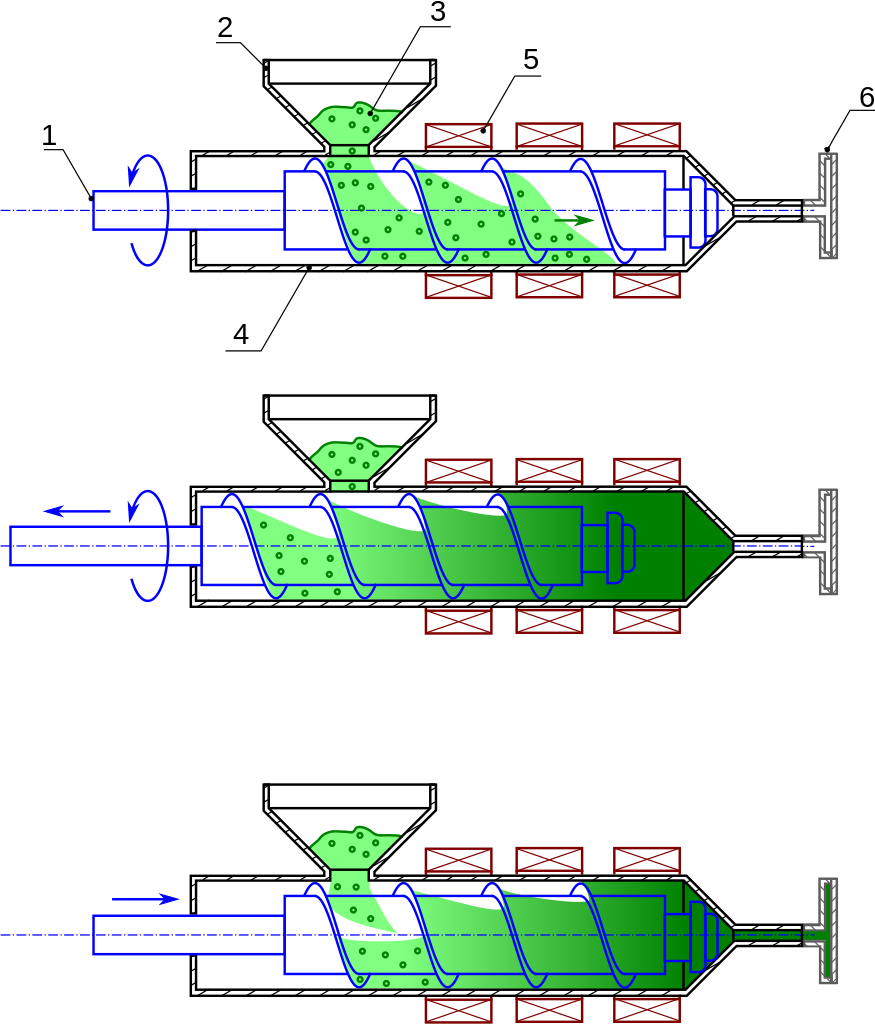
\includegraphics[height=0.5\textheight]{Bilder/Optische_Datentraeger_Die_Compact_Disc/Herstellung/cdspritz.png}
                    \caption[Spritzgussverfahren \newline \url{https://upload.wikimedia.org/wikipedia/commons/thumb/2/23/Principe_moulage_injection_polymere.svg/899px-Principe_moulage_injection_polymere.svg.png} (zuletzt aufgerufen am 11.08.2015)]{Spritzgussverfahren: 1. Schnecke, 2. Einfülltrichter, 3. Granulat, 4. Plastifizier\-zylinder, 5. Heizelemente, 6. CD-Form inklusive Metallmatrize}
                    \label{fig:cdspritz}
                \end{center}
            \end{minipage}
        \end{center}
    \end{figure}
}{}

\subsection{Trägermaterial: Polycarbonat}
\label{subsec:cdpc}

\subsubsection{Vorteile von Polycarbonat gegenüber anderen Materialien}

Polycarbonat wurde 1953 von dem bei der Firma Bayer angestellten Chemiker
Hermann Schnell entdeckt. Der neue Kunststoff wurde später unter dem Namen
Makrolon\textsuperscript{\textregistered} vermarktet. \cite{cuzpc}

Nachdem Philips seinen ersten CD-Prototypen hergestellt hatte, suchte man nach
einem Trägermaterial, welches für die Massenproduktion mittels
Spritzgussverfahren geeignet ist. Hierfür ist Polycarbonat nahezu perfekt. Die
niedrige Viskosität ermöglicht eine fehlerfreie Übertragung der Pitstruktur von
der Matrize auf die Polycarbonatscheibe. Hohe Transparenz und ein konstanter
Brechungsindex\footnote{Verhältnis der Lichtgeschwindigkeit und der
Ausbreitungsgeschwindigkeit von Licht im untersuchten Material} erlauben ein
unabgeschwächtes Durchdringen des Laserstrahls durch das Trägermaterial. Eine
hohe Erweichungstemperatur bei ca. 149°C \cite{cuzpc2} und Resistenz gegenüber
physikalischen Belastungen machen Polycarbonat alltagstauglich. \cite{cfcd}

\autoref{fig:cdpcpmma} vergleicht Polycarbonat (PC) und Polymethylmethacrylat
(PMMA) in Bezug auf Eigenschaften, die für die Herstellung und Benutzung der CD
relevant sind. Die Eignung nimmt in den jeweiligen Punkten von innen nach außen
zu. PMMA schneidet in fast allen Punkten mit Bestnoten ab, ist jedoch in den
Kategorien Wärmeformbeständigkeit und Wasseraufnahme PC unterlegen. Dies sowie
das gute Abschneiden bei den anderen Eigenschaften macht Polycarbonat zum
bevorzugten Kunststoff für die CD-Produktion.

\ifthenelse{\boolean{showPics}}{
    \begin{figure}[h]
        \begin{center}
            \begin{minipage}[t]{\textwidth}
                \begin{center}
                    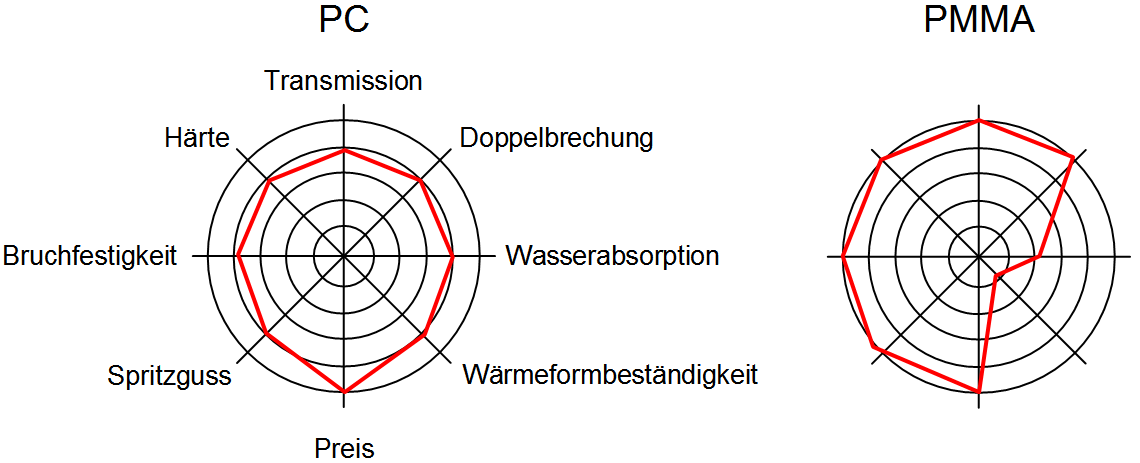
\includegraphics[height=0.1\textheight]{Bilder/Optische_Datentraeger_Die_Compact_Disc/Traegermaterial_Polycarbonat/cdpcpmma.png}
                    \caption[Vergleich zwischen PC und PMMA \newline Roth, Klaus: CD, DVD \& Co.: Die Chemie der schillernden Scheiben, in: Chemie in unserer Zeit (41/2007), S. 337]{Vergleich zwischen PC und PMMA}
                    \label{fig:cdpcpmma}
                \end{center}
            \end{minipage}
        \end{center}
    \end{figure}
}{}

\subsubsection{Polykondensation von Polycarbonat}

Polycarbonat kann entweder über eine Umesterung oder über eine
Grenzflächenkondensation hergestellt werden \cite{cuzpe}. Beide Reaktionen sind
Sonderformen der Polykondensation, da ein Polyester entsteht, sich aber kein
Wasser abspaltet. Polycarbonat selbst ist ein lineares Makromolekül und zählt
somit zu den Thermoplasten, da die beiden Edukte jeweils über zwei funktionale
Gruppen verfügen.

\paragraph{Umesterung} Bei der Umesterung kommen die geschmolzenen Monomere
Bisphenol A und Diphenylcarbonat zum Einsatz. \autoref{rec:diphenylcarbonat}
zeigt die Herstellung von Diphenylcarbonat aus Phenol und Phosgen unter
Abspaltung von Salzsäure \cite{cuzpe}. Bisphenol A und Diphenylcarbonat
reagieren in \autoref{rec:polycarbonat} zu Polycarbonat. Zumeist wird die
Reaktion alkalisch katalysiert und findet bei Temperaturen zwischen 250 - 350°C
statt \cite{pop}. Die beiden Monomere sind zu gleichen Teilen in dem Copolymer
vertreten, da sie auf alternierende Weise angeordnet sind. Die Reaktion endet
wenn keine Monomere mehr vorhanden sind.

\ifthenelse{\boolean{showPics}}{
    \begin{figure}[H]
        \begin{center}
            \footnotesize
            \setatomsep{1.7em}

            \chemname{$2$ \chemfig{*6(-=-(-OH)=-=)}}{Phenol}
            \chemsign{+}
            \chemname{\chemfig{C(=[:90]\lewis{13,O})(-[:210,1.25pt]\lewis{357,Cl})(-[:330,1.25pt]\lewis{157,Cl})}}{Phosgen}
            \chemrel{->}
            \chemname{\chemfig{C(=[:90]\lewis{13,O})(-[:210,1.25pt]\lewis{57,O}-[:150](*6(-=-=-=)))(-[:330,1.25pt]\lewis{57,O}-[:30](*6(-=-=-=)))}}{Diphenylcarbonat}
            \chemsign{+}
            \chemname{$2$ \chemfig{HCl}}{Salzsäure}

            \caption{Herstellung von Diphenylcarbonat}
            \label{rec:diphenylcarbonat}
        \end{center}
    \end{figure}

    \begin{figure}[H]
        \begin{center}
            \footnotesize
            \setatomsep{1.7em}

            \chemname{$n$ \chemfig{C(-[4]*6(-=-(-HO)=-=))(-[2]CH_3)(-[6]CH_3)(-[0]*6(-=-(-OH)=-=))}}{Bisphenol A}
            \chemsign{+}
            \chemname{$n$ \chemfig{C(=[:90]\lewis{13,O})(-[:210,1.25pt]\lewis{57,O}-[:150](*6(-=-=-=)))(-[:330,1.25pt]\lewis{57,O}-[:30](*6(-=-=-=)))}}{Diphenylcarbonat}

            \vspace{10pt}

            \chemrel{->}
            \chemname{\chemfig{C(-[4]*6(-=-(-\lewis{26,O}-[@{op,0.5}]H)=-=))(-[2]CH_3)(-[6]CH_3)(-[0]*6(-=-(-\lewis{26,O}-C(=[2]\lewis{13,O})-[@{cl,0.75}]\lewis{26,O}-(*6(-=-=-=)))=-=))}}{Polycarbonat}
            \makebraces[23pt,23pt]{n}{op}{cl}
            \chemsign{+}
            \chemname{$(2n-1)$ \chemfig{*6(-=-(-OH)=-=)}}{Phenol}

            \caption{Umesterung: Polykondensation von Polycarbonat}
            \label{rec:polycarbonat}
        \end{center}
    \end{figure}
}{}

Die \autoref{rec:deprotonierung} bis \autoref{rec:abspaltung} zeigen den ersten
Umesterungsvorgang, also den Beginn des Kettenwachstums im basischen Milieu. Als
erstes findet die Deprotonierung von Bisphenol A (siehe
\autoref{rec:deprotonierung}) statt. Dabei spaltet sich ein Proton
(H\textsuperscript{+}) von einer der Hydroxygruppen ab und lagert sich an das
Hydroxidion an. Durch diesen Vorgang wird das Bisphenol A negativ geladen und
das Hydroxidion wird zu Wasser protoniert. Die Umesterung selbst beginnt mit dem
nukleophilen Angriff (siehe \autoref{rec:nukleophilerangriff}) des Bisphenol
A-Anions auf das Diphenylcarbonat. Dabei lagert sich das negativ geladene
Sauerstoffatom an das positiv polarisierte Kohlenstoffatom des Diphenylcarbonats
an. Aufgrund der Vierbindigkeit des C-Atoms \glqq klappt\grqq{} eine der
Elektronenpaarbindungen des doppeltgebundenen Sauerstoffatoms zu dem O-Atom.
Durch weiteres \glqq Herumklappen\grqq{} von Elektronenpaarbindungen, wie in
\autoref{rec:abspaltung} dargestellt, kann eine der Phenylgruppen in Form eines
Phenolations abgespalten werden. Dabei bildet sich die Doppelbindung zwischen
dem Sauerstoff- und dem Kohlenstoffatom zurück und die Bindung zwischen einer
der beiden Phenylgruppen und dem C-Atom \glqq klappt\grqq{} zum O-Atom. Das
entstandene Dimer kann einen eigenen nukleophilen Angriff auf ein
Diphenylcarbonat oder auf ein ebenfalls durch Umesterung entstandenes Oligomer
bzw. Polymer durchführen, vorausgesetzt die verbliebene Hydroxygruppe wurde
zuvor deprotoniert. Alternativ kann es selbst durch ein Bisphenol A-Anion oder
durch ein deprotoniertes Oligomer bzw. Polymer angegriffen werden. In beiden
Fällen kommt es zu einer Umesterung und die Kette wächst durch die Wiederholung
dieser Schritte zu einem Polycarbonat an.

\ifthenelse{\boolean{showPics}}{
    \begin{figure}[H]
        \begin{center}
            \footnotesize
            \setatomsep{1.7em}

            \chemname{\chemfig{C(-[4]*6(-=-(-HO)=-=))(-[2]CH_3)(-[6]CH_3)(-[0]*6(-=-(-O@{pr1}H)=-=))}}{Bisphenol A}
            \chemsign{+}
            \chemname{\chemfig{@{ak1}OH(-[:135,.5,,,draw=none]\fsscrm)}}{Hydroxidion}
            \chemmove[->,shorten <=2pt]{\draw[shorten >=2pt](pr1).. controls +(90:1cm) and +(90:1cm).. (ak1);}
            \chemrel{->}
            \chemname{\chemfig{C(-[4]*6(-=-(-HO)=-=))(-[2]CH_3)(-[6]CH_3)(-[0]*6(-=-(-\lewis{026,O}(-[:45,.7,,,draw=none]\fsscrm))=-=))}}{Bisphenol A-Anion}
            \chemsign{+}
            \chemname{\chemfig{H_2O}}{Wasser}

            \caption{Umesterung: Deprotonierung von Bisphenol A durch Hydroxidionen}
            \label{rec:deprotonierung}
        \end{center}
    \end{figure}

    \begin{figure}[H]
        \begin{center}
            \footnotesize
            \setatomsep{1.7em}

            \chemname{\chemfig{C(-[4]*6(-=-(-HO)=-=))(-[2]CH_3)(-[6]CH_3)(-[0]*6(-=-(-@{np2}\lewis{026,O}(-[:45,.7,,,draw=none]\fsscrm))=-=))}}{Bisphenol A-Anion}
            \chemsign{+}
            \chemname{\chemfig{@{ep2}C(-[:25,.7,,,draw=none]\fdelp)(=[@{db2}:90]@{o2}\lewis{13,O})(-[:210]\lewis{57,O}-[:150](*6(-=-=-=)))(-[:330]\lewis{57,O}-[:30](*6(-=-=-=)))}}{Diphenylcarbonat}
            \chemmove[->,shorten <=2.5pt]{
                \draw[shorten >=2.5pt](np2).. controls +(90:1cm) and +(135:2.5cm).. (ep2);
                \draw[shorten >=6pt](db2).. controls +(0:1cm) and +(90:1cm).. (o2);}

            \vspace{10pt}

            \chemrel{->}
            \chemname{\chemfig{C(-[4]*6(-=-(-HO)=-=))(-[2]CH_3)(-[6]CH_3)(-[0]*6(-=-(-\lewis{26,O}-C(-[2]\lewis{024,O}(-[:45,.7,,,draw=none]\fsscrm))(-[0]\lewis{26,O}-(*6(=-=-=-)))(-[6]\lewis{04,O}-[6](*6(=-=-=-))))=-=))}}{}

            \caption{Umesterung: nukleophiler Angriff}
            \label{rec:nukleophilerangriff}
        \end{center}
    \end{figure}

    \begin{figure}[H]
        \begin{center}
            \footnotesize
            \setatomsep{1.7em}

            \chemname{\chemfig{C(-[4]*6(-=-(-HO)=-=))(-[2]CH_3)(-[6]CH_3)(-[0]*6(-=-(-\lewis{26,O}-C(-[@{ndb3}2]@{o3}\lewis{024,O}(-[:45,.7,,,draw=none]\fsscrm))(-[0]\lewis{26,O}-(*6(=-=-=-)))(-[@{b3}6]@{p3}\lewis{04,O}-[6](*6(=-=-=-))))=-=))}}{}
            \chemmove[->,shorten <=2.5pt]{
                \draw[shorten >=2.5pt](b3).. controls +(0:1cm) and +(315:1cm).. (p3);
                \draw[shorten >=2.5pt](o3).. controls +(0:0.5cm) and +(0:0.5cm).. (ndb3);}

            \vspace{10pt}

            \chemrel{->}
            \chemnameinit{}
            \chemname{\chemfig{C(-[4]*6(-=-(-HO)=-=))(-[2]CH_3)(-[6]CH_3)(-[0]*6(-=-(-\lewis{26,O}-C(=[2]\lewis{13,O})-\lewis{26,O}-(*6(-=-=-=)))=-=))}}{Dimer}
            \chemsign{+}
            \chemname{\chemfig{*6(-=-(-\lewis{137,O}(-[:0,.7,,,draw=none]\fsscrm))=-=)}}{Phenolation}

            \caption{Umesterung: Abspaltung eines Phenolation}
            \label{rec:abspaltung}
        \end{center}
    \end{figure}
}{}

\paragraph{Grenzflächenkondensation} Die zweite Möglichkeit, Polycarbonat
herzustellen, besteht in der Grenzflächenkondensation. Hierfür werden Bisphenol
A in eine wässrige basische Lösung sowie Phosgen in eine organische Lösung
versetzt \cite{cuzpe}. Als Base kann z.B. Natriumhydroxid dienen. Durch die
Deprotonierung von Bisphenol A durch Natriumhydroxid (siehe
\autoref{rec:deprotonierung2}) enthält die wässrige Lösung Bisphenol A-Anionen
und Natriumionen. Durch die negative Ladung des Bisphenol A erhöht sich dessen
Reaktivität und begünstigt das Kettenwachstum. \autoref{rec:polycarbonat2} zeigt
die Polymerbildung durch eine Polykondensation zwischen den Bisphenol A-Anionen
und Phosgen an der Grenzfläche zwischen der basischen und organischen Phase.
Dabei spalten sich Chloridionen ab, welche mit den Natriumionen als
Natriumchlorid ausfallen. Die Reaktion in \autoref{rec:polycarbonat2} findet in
Form eines nukleophilen Angriffes statt, der dem zwischen dem Bisphenol A-Anion
und Diphenylcarbonat in \autoref{rec:nukleophilerangriff} und
\autoref{rec:abspaltung} ähnelt (das Phosgen übernimmt die Funktion des
Diphenylcarbonats und es spaltet sich statt eines Phenolations ein Chloridion
ab). Durch Verdampfen des organischen Lösungsmittels lässt sich das Polycarbonat
gewinnen \cite{garoo}.

\ifthenelse{\boolean{showPics}}{
    \begin{figure}[H]
        \begin{center}
            \footnotesize
            \setatomsep{1.7em}

            \chemname{\chemfig{C(-[4]*6(-=-(-HO)=-=))(-[2]CH_3)(-[6]CH_3)(-[0]*6(-=-(-OH)=-=))}}{Bisphenol A}
            \chemsign{+}
            \chemname{$2$ \chemfig{Na(-[:45,.5,,,draw=none]\fsscrp)(-[:0,1.2,,,draw=none])OH(-[:135,.5,,,draw=none]\fsscrm)}}{Natriumhydroxid}

            \vspace{10pt}

            \chemrel{->}
            \chemname{\chemfig{C(-[4]*6(-=-(-\lewis{246,O}(-[:135,.7,,,draw=none]\fsscrm)(-[:180,1.4,,,draw=none])Na(-[:45,.6,,,draw=none]\fsscrp))=-=))(-[2]CH_3)(-[6]CH_3)(-[0]*6(-=-(-\lewis{026,O}(-[:45,.7,,,draw=none]\fsscrm)(-[:0,1.4,,,draw=none])Na(-[:135,.6,,,draw=none]\fsscrp))=-=))}}{Bisphenol A-Anion, Natriumionen}
            \chemsign{+}
            \chemname{$2$ \chemfig{H_2O}}{Wasser}

            \caption{Grenzflächenkondensation: Deprotonierung von Bisphenol A durch Natriumhydroxid}
            \label{rec:deprotonierung2}
        \end{center}
    \end{figure}

    \begin{figure}[H]
        \begin{center}
            \footnotesize
            \setatomsep{1.7em}

            \chemname{$n$ \chemfig{C(-[4]*6(-=-(-\lewis{246,O}(-[:135,.7,,,draw=none]\fsscrm)(-[:180,1.4,,,draw=none])Na(-[:45,.6,,,draw=none]\fsscrp))=-=))(-[2]CH_3)(-[6]CH_3)(-[0]*6(-=-(-\lewis{026,O}(-[:45,.7,,,draw=none]\fsscrm)(-[:0,1.4,,,draw=none])Na(-[:135,.6,,,draw=none]\fsscrp))=-=))}}{Bisphenol A-Anion, Natriumionen}
            \chemsign{+}
            \chemname{$n$ \chemfig{C(=[:90]\lewis{13,O})(-[:210,1.25pt]\lewis{357,Cl})(-[:330,1.25pt]\lewis{157,Cl})}}{Phosgen}

            \vspace{10pt}

            \chemrel{->}
            \chemname{\chemfig{C(-[4]*6(-=-(-\lewis{26,O}-[@{op,0.75}])=-=))(-[2]CH_3)(-[6]CH_3)(-[0]*6(-=-(-\lewis{26,O}-C(=[2]\lewis{13,O})-[@{cl,0.75}])=-=))}}{Polycarbonat}
            \makebraces[23pt,23pt]{n}{op}{cl}
            \chemsign{+}
            \chemname{$2n$ \chemfig{Na(-[:45,.6,,,draw=none]\fsscrp)(-[:0,1.3,,,draw=none])Cl(-[:135,.6,,,draw=none]\fsscrm)}}{Natriumchlorid}

            \caption{Grenzflächenkondensation: Polykondensation von Polycarbonat}
            \label{rec:polycarbonat2}
        \end{center}
    \end{figure}
}{}

\subsubsection{Nachweis der hohen Lichtdurchlässigkeit sowie der einfachen Weiterverarbeitung von Polycarbonat}

Um die hohe Lichtdurchlässigkeit und die einfache Weiterverarbeitung von
Polycarbonat nachzuweisen, wird der folgende Versuch durchgeführt.\\

\par

Material:
\begin{compactitem}
    \item handelsübliche CD, Schere, 2 Glasschalen, Plätzchenform, Pinzette, Aluminium\-folie, Heizplatte
    \item Chemikalie: \\[5pt]
    \begin{tabular}{ll}
    Salpetersäure: & Sicherheitshinweis CAS Nr. 7697-37-2 \\
    & (brandfördernder und ätzender Stoff) \\
    \end{tabular}
\end{compactitem}~\par

\\Schutzvorkehrungen:
\begin{compactitem}
    \item Abzug, Schutzkleidung, Handschuhe, Schutzbrille
\end{compactitem}~\par

\\Versuchsablauf \cite{cdversuch}:
\begin{compactenum}
    \item Die CD wird in eine der Glasschalen gelegt und mit Salpetersäure übergossen (siehe \autoref{fig:cdsalpeter}). Dies muss unter einem Abzug geschehen, da nitrose Gase entstehen.
    \item Nach kurzer Zeit \glqq quellen\grqq{} die Lack- und die Aluminiumschicht auf (siehe \autoref{fig:cdquillt}) und lassen sich mithilfe der Pinzette entfernen.
    \item Die \glqq gehäutete\grqq{} CD wird nun in die zweite Glasschale gelegt und vorsichtig unter dem Wasserhahn abgespült. \autoref{fig:cdblank} zeigt die resultierende Polycarbonatscheibe.
    \item Die Lichtdurchlässigkeit der Polycarbonatscheibe wird überprüft, indem die Scheibe in ein CD-Laufwerk eingelegt wird.
    \item Die Polycarbonatscheibe wird anschließend in maximal 1 cm² kleine Stücke zerschnitten (siehe \autoref{fig:cdzerschnitten}).
    \item Die Polycarbonatstücke werden ca. 1 cm hoch in die Plätzchenform gefüllt. Diese befindet sich auf einer mit Aluminiumfolie bedeckten Heizplatte (siehe \autoref{fig:cdschmelzen}).
    \item Die Heizplatte wird auf über 250°C erhitzt. Sobald das Polycarbonat geschmolzen ist, wird die Heizplatte ausgeschaltet.
    \item Nach dem Abkühlen wird das \glqq Polycarbonatplätzchen\grqq{} aus der Form gebrochen (siehe \autoref{fig:cdplaetzchen}).
\end{compactenum}

\ifthenelse{\boolean{showPics}}{
    \begin{figure}[H]
        \begin{center}
            \begin{minipage}[t]{0.45\textwidth}
                \begin{center}
                    \includegraphics[height=0.1\textheight]{Bilder/Optische_Datentraeger_Die_Compact_Disc/Traegermaterial_Polycarbonat/cdsalpeter.png}
                    \caption[CD in Salpetersäure]{CD in Salpetersäure}
                    \label{fig:cdsalpeter}
                \end{center}
            \end{minipage}
            \hspace{0.025\textwidth}
            \begin{minipage}[t]{0.45\textwidth}
                \begin{center}
                    \includegraphics[height=0.1\textheight]{Bilder/Optische_Datentraeger_Die_Compact_Disc/Traegermaterial_Polycarbonat/cdquillt.png}
                    \caption[aufgequollene Lack- und Aluminiumschicht]{\glqq aufgequollene\grqq{} Lack- und Aluminiumschicht}
                    \label{fig:cdquillt}
                \end{center}
            \end{minipage}
        \end{center}
    \end{figure}

    \begin{figure}[H]
        \begin{center}
            \begin{minipage}[t]{0.45\textwidth}
                \begin{center}
                    \includegraphics[height=0.1\textheight]{Bilder/Optische_Datentraeger_Die_Compact_Disc/Traegermaterial_Polycarbonat/cdblank.png}
                    \caption[Polycarbonatscheibe]{Polycarbonatscheibe}
                    \label{fig:cdblank}
                \end{center}
            \end{minipage}
            \hspace{0.025\textwidth}
            \begin{minipage}[t]{0.45\textwidth}
                \begin{center}
                    \includegraphics[height=0.1\textheight]{Bilder/Optische_Datentraeger_Die_Compact_Disc/Traegermaterial_Polycarbonat/cdzerschnitten.png}
                    \caption[Polycarbonatstücke]{Polycarbonatstücke}
                    \label{fig:cdzerschnitten}
                \end{center}
            \end{minipage}
        \end{center}
    \end{figure}

    \begin{figure}[H]
        \begin{center}
            \begin{minipage}[t]{0.45\textwidth}
                \begin{center}
                    \includegraphics[height=0.1\textheight]{Bilder/Optische_Datentraeger_Die_Compact_Disc/Traegermaterial_Polycarbonat/cdschmelzen.png}
                    \caption[Heizplatte mit Plätzchenform]{Heizplatte mit Plätzchenform}
                    \label{fig:cdschmelzen}
                \end{center}
            \end{minipage}
            \hspace{0.025\textwidth}
            \begin{minipage}[t]{0.45\textwidth}
                \begin{center}
                    \includegraphics[height=0.1\textheight]{Bilder/Optische_Datentraeger_Die_Compact_Disc/Traegermaterial_Polycarbonat/cdplaetzchen.png}
                    \caption[\glqq Polycarbonatplätzchen\grqq{}]{\glqq Polycarbonatplätzchen\grqq{}}
                    \label{fig:cdplaetzchen}
                \end{center}
            \end{minipage}
        \end{center}
    \end{figure}
}{}

Ergebnisse des Versuchs:
\begin{enumerate*}
    \item Hohe Lichtdurchlässigkeit: Wird die \glqq gehäutete\grqq{} CD in das CD-Laufwerk eines Computers eingelegt, wird diese nicht erkannt, da der Laserstrahl ungehindert durch die Polycarbonatscheibe geht. Dies zeigt, dass die Aluminiumschicht für die Reflexion des Laserstrahls verantwortlich ist.
    \item Einfache Weiterverarbeitung: Die Polycarbonatstücke lassen sich ohne großen Aufwand und innerhalb kurzer Zeit in eine neue Form schmelzen. Die Qualitätsminderung liegt an Verschmutzungen und Lufteinschlüssen, die aufgrund der primitiven Einschmelzmethode unvermeidbar sind.
\end{enumerate*}


\section{Optische Wellenleiter - Die polymer optische Faser}
\label{sec:pof}

\subsection{Allgemeines}
\label{subsec:pofallgemeines}

Optische Wellenleiter, auch Lichtwellenleiter genannt, verwenden Licht zur
Übertragung von Informationen. Dies ermöglicht eine schnellere Datenübertragung
als mit Kupferkabeln. Glasfaserkabel werden aufgrund ihrer hohen Reichweite von
mehreren Kilometern und der hohen Übertragungsleistung von bis zu 32 Gigabit/s
pro Kabel für die Verbindung von Städten und Kontinenten eingesetzt. Die
Anbindung von Gebäuden und Wohnungen an das Glasfaserkabelnetz ist mittlerweile
ein erklärtes Ziel der Telekommunikationsunternehmen. Durch Projekte wie \glqq
Fiber to the Home\grqq{} oder \glqq Fiber to the Building\grqq{} sollen
Privatpersonen und Unternehmen von hohen Übertragungsgeschwindigkeiten
profitieren. Für die Verlegung in Gebäuden sind Glasfaserkabel jedoch nur
bedingt geeignet, da Fachpersonal mit Spezialwerkzeug erforderlich ist. Polymer
optische Fasern (POF) bieten sich hier als kostengünstige Alternative an. Sie
lassen sich einfach und platzsparend verlegen (der Durchmesser beträgt ca. 1 mm)
und auf kurzen Distanzen \nolbreaks{(< 100 m)} können Datenraten von bis zu 40
Gigabit/s erreicht werden \cite{pofacgif}. Kabel aus polymer optischen Fasern
werden außerdem in Flugzeugen, Zügen, Automobilen und Industrieanlagen
eingesetzt. \autoref{fig:pofgrund} zeigt die Gründe für die Verwendung in dem
jeweiligen Bereich. Die Größe des Kreises in der jeweiligen Zelle gibt die
Relevanz des Kriteriums an. \cite{poflan}

\ifthenelse{\boolean{showPics}}{
    \begin{figure}[h]
        \begin{center}
            \begin{minipage}[t]{\textwidth}
                \begin{center}
                    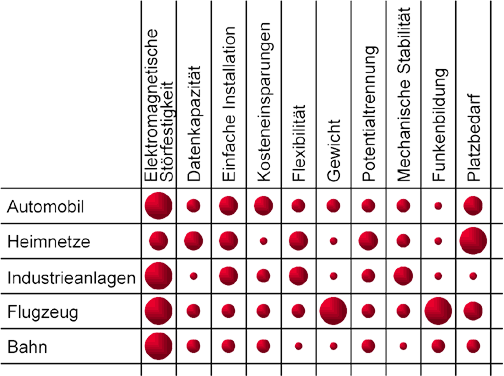
\includegraphics[height=0.2\textheight]{Bilder/Optische_Wellenleiter_Die_Polymer_Optische_Faser/Allgemeines/pofgrund.png}
                    \caption[Gründe für die Verwendung von POF-Kabel \newline \url{http://www.pofac.fh-nuernberg.de/pofac/de/was_sind_pof/images/warum_pof.png} (zuletzt aufgerufen am 19.09.2015)]{Gründe für die Verwendung von POF-Kabel}
                    \label{fig:pofgrund}
                \end{center}
            \end{minipage}
        \end{center}
    \end{figure}
}{}

Elektromagnetische Strahlung, elektrische Felder und Magnetfelder
beeinträchtigen den Fluss von Elektronen in Kupferkabeln, jedoch nicht den von
Lichtstrahlen in einem Lichtwellenleiter. Daher kommen polymer optische Fasern
überall dort zum Einsatz, wo eine ungestörte Datenübertragung wichtig ist. In
Flugzeugen reduziert das geringe Gewicht von POF-Kabeln den Treibstoffverbrauch
und damit die Betriebskosten. Zudem wird Funkenbildung vermieden, da polymer
optische Fasern keine Elektronen sondern Licht übertragen. POF-Kabel werden auch
in Krankenhäusern eingesetzt, da sie keine elektromagnetische Strahlung
emittieren und deshalb empfindliche Messgeräte nicht stören.

\subsection{Funktionsweise}
\label{subsec:poffunktionsweise}

Informationen werden mittels Intensitätsmodulationen der Lichtstrahlen
übertragen. Dabei wird das Licht durch eine transparente Kern, welcher von einem
Mantel umgeben ist, gesendet (siehe \autoref{fig:pofprinzip}). Die Brechzahl $n$
des Kernes ist dabei größer als die des Mantels. Dies ermöglicht eine
Totalreflexion des Lichts am Übergang von Kern zum Mantel.
\autoref{fig:poflichtausbreitung} zeigt zwei mögliche Ausbreitungen von
Lichtimpulsen in einer polymer optischen Faser. Die Laufzeiten der beiden
Strahlen untrscheidet sich jedoch, da der hellblaue Strahl einen kürzeren Weg
für die Durchquerung des abgebildeten Leiterstückes als der grüne Strahl
zurücklegt. Die Laufzeitunterschied zwischen den Lichtstrahlen beschränken die
Bandbreite des Kabels. Die Bitraten erhöhen sich bei kürzeren Strecken, da sich
die Unterschiede zwischen den Laufzeiten verringern. Durch die Totalreflektion
kann das Licht auch durch Biegungen geleitet werden.

%Die Laufzeitunterschied zwischen dem schnellsten Strahl (ohne eine Reflektion) und dem langsamsten Strahl (die meistes Reflektion\footnote{Die Totalreflexion ist ab einem bestimmten Einfallswinkel nicht mehr möglich. Dadurch wird die maximale Reflexionszahl auf einer gewissen Strecke beschränkt}) bestimmt die Bandbreite des Kabels.

\begin{figure}[h]
    \begin{center}
        \begin{minipage}[t]{0.4\textwidth}
            \begin{center}
                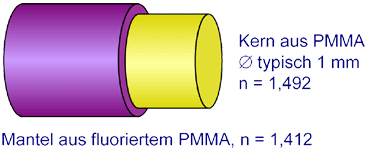
\includegraphics[height=0.4\textwidth]{Bilder/Optische_Wellenleiter_Die_Polymer_Optische_Faser/Funktionsweise/pofprinzip.png}
                \caption[Aufbau eines Kabels aus POF \newline \url{http://www.pofac.fh-nuernberg.de/pofac/de/was_sind_pof/images/pof_prinzip.png}]{Aufbau eines Kabels aus POF}
                \label{fig:pofprinzip}
            \end{center}
        \end{minipage}
        \hspace{0.025\textwidth}
        \begin{minipage}[t]{0.4\textwidth}
            \begin{center}
                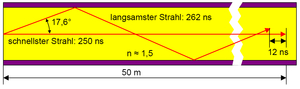
\includegraphics[height=0.1\textheight]{Bilder/Optische_Wellenleiter_Die_Polymer_Optische_Faser/Funktionsweise/poflichtausbreitung.png}
                \caption[Ausbreitung von Licht in einem optischen Wellenleiter \newline \url{http://www.itwissen.info/bilder-klein/lwl-mit-verschiedenen-moden.png}]{Ausbreitung von Licht in einem optischen Wellenleiter} %TODO: better resolution
                \label{fig:poflichtausbreitung}
            \end{center}
        \end{minipage}
    \end{center}
\end{figure}

\autoref{fig:pofdaempfung} zeigt die Dämpfungsfenster einer polymer optischen
Faser. Diese liegen bei den Farben grün, gelb und rot. Um die Intensitätsabnahme
möglichst gering zu halten und damit die Reichweite zu erhöhen werden
Wellenlängen für die Lichtimpulse gewählt, die in den Dämpfungsfenstern liegen.

\begin{figure}[h]
    \begin{center}
        \begin{minipage}[t]{0.4\textwidth}
            \begin{center}
                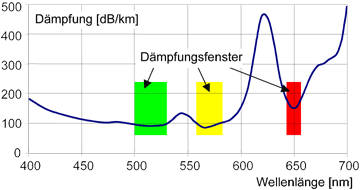
\includegraphics[height=0.1\textheight]{Bilder/Optische_Wellenleiter_Die_Polymer_Optische_Faser/Funktionsweise/pofdaempfung.png}
                \caption[Dämpfungsfenster bei einer polymer optischen Faser \newline \url{http://www.pofac.fh-nuernberg.de/pofac/de/was_sind_pof/images/pmma_daempfung.png}]{Dämpfungsfenster bei einer polymer optischen Faser}
                \label{fig:pofdaempfung}
            \end{center}
        \end{minipage}
    \end{center}
\end{figure}

\subsection{Brechzahlprofile der Kernmaterialien}
\label{subsec:pofbrechzahlprofile}

Um die Bandbreite von einem POF-Kabel zu erhöhen kommen Faser zum Einsatz deren
Brechzahlen modifiziert wurden. Dies geschieht durch die Wahl des Kernmaterials oder durch spezielle Fertigungsverfahren. Durch die Modifikation der Brechzahlen wird der Weg des Lichts innerhalb des Kernes beeinflusst.

\subsubsection{Stufenindexprofil (SI-POF)}

Der Stufenindex ist durchsatzschwächste Brechzahlprofil (ca. 100 Megabit/s auf
100 m, spezielle Übertragungsverfahren erlauben Bitraten im Bereich von 1
Gigabit/s). Als Kernmaterial wird Polymethylmethacrylat mit einem Durchmesser
von ca. 1 mm, welcher von einem ca. 10 µm Mantel umgeben ist, eingesetzt
\cite{pofacsi}. \autoref{fig:pofsi} fasst den Aufbau und die Lichtausbreitung
zusammen. Die Spalte mit Brechungsindex als Überschrift stellt den Verlauf
dieses grafisch dar. Beim Stufenindexprofil steigen die Brechzahlen beim
Übergang vom Mantel zum Kern abrupt an. Dies hat die schon erwähnte
Totalreflexion an der Kerngrenze, welche man in der Spalte Querschnitt erkennen
kann, zur Folge.

\begin{figure}[h]
    \begin{center}
        \begin{minipage}[t]{0.4\textwidth}
            \begin{center}
                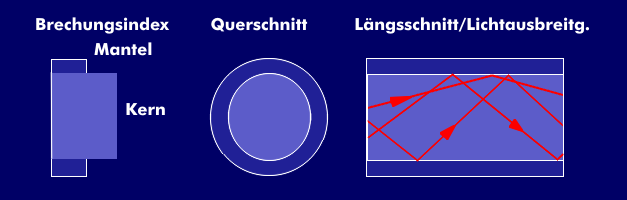
\includegraphics[width=0.9\textwidth]{Bilder/Optische_Wellenleiter_Die_Polymer_Optische_Faser/Brechzahlprofile/pofsi.png}
                \caption[Aufbau des Stufenindexprofils \newline \url{http://www.itwissen.info/bilder/aufbau-und-brechungsprofil-der-stufenindex-profilfaser.png} (zuletzt aufgerufen am 19.09.2015)]{Aufbau des Stufenindexprofils}
                \label{fig:pofsi}
            \end{center}
        \end{minipage}
        \hspace{0.025\textwidth}
        \begin{minipage}[t]{0.4\textwidth}
            \begin{center}
                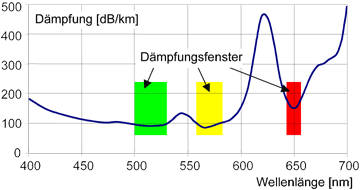
\includegraphics[height=0.1\textheight]{Bilder/Optische_Wellenleiter_Die_Polymer_Optische_Faser/Funktionsweise/pofdaempfung.png}
                \caption[Dämpfungsfenster bei einer polymer optischen Faser \newline \url{http://www.pofac.fh-nuernberg.de/pofac/de/was_sind_pof/images/pmma_daempfung.png} (zuletzt aufgerufen am 19.09.2015)]{Dämpfungsfenster beim Stufenprofil}
                \label{fig:pofdaempfung}
            \end{center}
        \end{minipage}
    \end{center}
\end{figure}

\autoref{fig:pofdaempfung} zeigt die Dämpfungsfenster einer polymer optischen
Faser. Diese liegen bei den Farben grün, gelb und rot. Um die Intensitätsabnahme
möglichst gering zu halten und damit die Reichweite zu erhöhen werden
Wellenlängen für die Lichtimpulse gewählt, die in den Dämpfungsfenstern liegen.
Als Lichtquelle kann zum Beispiel eine LED verwendet werden und als Empfänger
kommen Photodetektoren zum Einsatz. Der geringe Preis und die robuste
Übertragung auf kurzen Strecken machen die SI-POF zu einer beliebten alternative
gegenüber von Kupferkabeln in Industrieanlagen oder in Fahrzeugen. \cite{poflee}

\subsubsection{Gradientenindexprofil (GI-POF)}

Das Gradientenindexprofil bittet mit bis zu 40 Gigabit/s auf 100m deutlich
höhere Bitraten als das Stufenindexprofil. Beim Gradientenindex nimmt der
Brechungsindex vom Mantel bis zur Mitte des Kern kontinuierlich zu (siehe
\autoref{fig:pofgi} Spalte Brechungsindex). \autoref{fig:pofgi} zeigt ebenfalls
in der Spalte Längsschnitt den daraus resultierenden Lichtstrahlenverlauf.
Dieser verläuft, im Gegensatz zu der geraden Lichtausbreitung beim Stufenindex,
sinusförmig. Der Kerndurchmesser der GI-POF ist mit ca. 100 µm um das 10fache
geringer als der einer SI-POF. Dadurch werden geringere Laufzeitunterschiede
ermöglicht und die Frequenz der Lichtimpulse kann erhöht werden. Außerdem wird
bei der GI-POF eine Dämpfung von unter 20 dB/km erreicht. Dies ist eine
ehrheblicher Verbesserung gegenüber der Dämpfung von SI-POF mit ca. 100 dB/km
(siehe \autoref{fig:pofgidaempfung}). Aus den beiden Gründen ist die Bandbreite
einer Faser mit Gradientenindex significant höher als die einer einer Faser mit
Stufenindex. Als Kernmaterial kann hier der Kunststoff
CYTOP\textsuperscript{\texttrademark} der Asahi Glass Co., Ltd. oder
Polymethylmethacrylat verwendet werden \cite{pofacgif}. Aufgrund der hohen
Bitraten und der Biegsamkeit werden GI-POF in \shorthandoff{"}"Local Area
Networks"\shorthandon{"} (LAN) und in Supercomputern eingesetzt \cite{poflee}.

\begin{figure}[h]
    \begin{center}
        \begin{minipage}[t]{0.4\textwidth}
            \begin{center}
                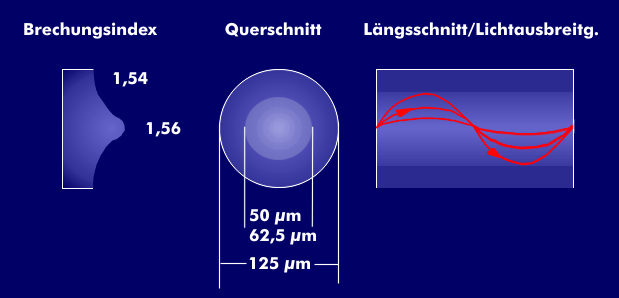
\includegraphics[width=0.9\textwidth]{Bilder/Optische_Wellenleiter_Die_Polymer_Optische_Faser/Brechzahlprofile/pofgi.png}
                \caption[Aufbau des Gradientenindexprofils \newline \url{http://www.itwissen.info/bilder/aufbau-und-brechungsprofil-der-gradientenfaser.png} (zuletzt aufgerufen am 19.09.2015)]{Aufbau des Gradientenindexprofils}
                \label{fig:pofgi}
            \end{center}
        \end{minipage}
        \hspace{0.025\textwidth}
        \begin{minipage}[t]{0.4\textwidth}
            \begin{center}
                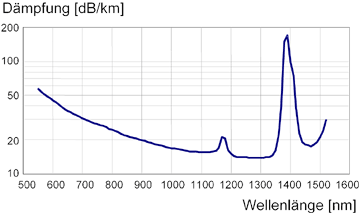
\includegraphics[height=0.1\textheight]{Bilder/Optische_Wellenleiter_Die_Polymer_Optische_Faser/Brechzahlprofile/pofgidaempfung.png}
                \caption[Dämpfung bei einer GI-POF \newline \url{http://www.pofac.fh-nuernberg.de/pofac/de/was_sind_pof/images/gradientenindex_daempfung.png} (zuletzt aufgerufen am 19.09.2015)]{Vergleich der Dämpfungswerte von GI-POF und SI-POF}
                \label{fig:pofgidaempfung}
            \end{center}
        \end{minipage}
    \end{center}
\end{figure}


\subsubsection{Weitere Profile}

Weitere Erhöhungen der Bandbreite werden durch mehrere Mäntel (siehe
\autoref{fig:pofdsi} \autoref{fig:pofmsi}, Reduzierung der Laufzeitunterschiede)
bzw. durch mehrere Kerne (siehe \autoref{fig:pofmc}, mehrere Lichtstrahlen
gleichzeitig) innerhalb eines Kabels erreicht. \autoref{fig:pofdsimc} zeigt eine
Kombination der beiden obigen Optimierungsmöglichkeiten.
\cite{pofacprofile}

\begin{figure}[h]
    \begin{center}
        \begin{minipage}[t]{0.4\textwidth}
            \begin{center}
                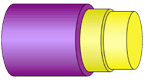
\includegraphics[height=0.1\textheight]{Bilder/Optische_Wellenleiter_Die_Polymer_Optische_Faser/Brechzahlprofile/pofdsi.png}
                \caption[\textit{Dual Step Index} - POF (zwei Mäntel, Stufenindex) \newline
                \url{http://www.pofac.fh-nuernberg.de/pofac/de/was_sind_pof/images/profil_dsi-pof.png} (zuletzt aufgerufen am 19.09.2015)]{\textit{Dual Step Index} - POF (zwei Mäntel, Stufenindex)}
                \label{fig:pofdsi}
            \end{center}
        \end{minipage}
        \hspace{0.025\textwidth}
        \begin{minipage}[t]{0.4\textwidth}
            \begin{center}
                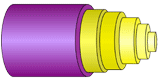
\includegraphics[height=0.1\textheight]{Bilder/Optische_Wellenleiter_Die_Polymer_Optische_Faser/Brechzahlprofile/pofmsi.png}
                \caption[\textit{Multi Step Index} - POF (mehrere Mäntel, Stufenindex) \newline
                \url{http://www.pofac.fh-nuernberg.de/pofac/de/was_sind_pof/images/profil_msi-pof.png} (zuletzt aufgerufen am 19.09.2015)]{\textit{Multi Step Index} - POF (mehrere Mäntel, Stufenindex)}
                \label{fig:pofmsi}
            \end{center}
        \end{minipage}
    \end{center}

    \begin{center}
        \begin{minipage}[t]{0.4\textwidth}
            \begin{center}
                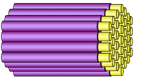
\includegraphics[height=0.1\textheight]{Bilder/Optische_Wellenleiter_Die_Polymer_Optische_Faser/Brechzahlprofile/pofmc.png}
                \caption[\textit{Multi Core} - POF (mehrere Kerne, Stufenindex) \newline
                \url{http://www.pofac.fh-nuernberg.de/pofac/de/was_sind_pof/images/profil_mc-pof.png} (zuletzt aufgerufen am 19.09.2015)]{\textit{Multi Core} - POF (mehrere Kerne, Stufenindex)}
                \label{fig:pofmc}
            \end{center}
        \end{minipage}
        \hspace{0.025\textwidth}
        \begin{minipage}[t]{0.4\textwidth}
            \begin{center}
                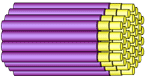
\includegraphics[height=0.1\textheight]{Bilder/Optische_Wellenleiter_Die_Polymer_Optische_Faser/Brechzahlprofile/pofdsimc.png}
                \caption[\textit{Dual Step Index - Multi Core} - POF (mehrere Kerne, zwei Mäntel, Stufenindex) \newline
                \url{http://www.pofac.fh-nuernberg.de/pofac/de/was_sind_pof/images/profil_dsi-mc-pof.png} (zuletzt aufgerufen am 19.09.2015)]{\textit{Dual Step Index - Multi Core} - POF (mehrere Kerne, zwei Mäntel, Stufenindex)}
                \label{fig:pofdsimc}
            \end{center}
        \end{minipage}
    \end{center}
\end{figure}

%CYTOP
\subsection{Material: Polymethylmethacrylat}
\label{subsec:pofpmma}

\subsubsection{Versuch: Herstellung von Polymethylmethacrylat}

Polymethylmethacrylat (PMMA) wurde erstmals von Otto Röhm 1928 hergestellt. Fünf
Jahre später wurde PMMA unter dem Namen
Plexiglas\textsuperscript{\textregistered} vermarktet. Die hohe optisch
Durchlässigkeit und das geringe Gewicht eignen PMMA für den Einsatz in der
Automobielindustrie. Gerade diese Eigenschaften sind ebenfalls ein Grund für die
Verwendung in POFs. \cite{pofwuppmma}

\subsubsection{Versuch: Vergleich zwischen der Synthese von Polymethylmethacrylat ohne Präpolymer und mit Präpolymer}
\label{subsubsec:versuchpmma}


\subsection{Herstellung von Optischen Wellenleitern}
\label{subsec:pofherstellungsverfahren}

\subsubsection{Herstellung einer SI-POF mittels Extrusion}

Für die Herstellung eines polymeren Wellenleiters mit Stufenindexprofil eignet
sich die kontinuirliche Extrusion (siehe \autoref{fig:pofsispinn}). Dabei werden
die Monomere samt Radikalstarter und Additiven in ein geheiztes
Polymerisationsgefäß (\textit{heating unit}) gegeben. Nachdem der Polymeranteil
in der Reaktionskammer hoch genug ist, werden diese in den Extruder gepumpt. Das
Polymer wird von dem Extruder in eine Spinndüse gedrückt. In der Spinndüse wird
der Kern des POFs geformt und mit einem Mantel aus dem Extruder mit dem
Mantelmaterial (\textit{cladding material}) versehen. Der Faden wird dann in
einer \textit{blow box} gekühlt, gedehnt (\textit{stretching}) und aufgerollt
(\textit{take-up}). Vorteilhaft bei diesem Verfahren ist die Eignung zur
Massenproduktion und die Reinheit des Kerns, da keine vorgefertigtes Granulat
verwendet wird. Ein Nachteil dagegen sind die hohen Kosten.

\begin{figure}[h]
    \begin{center}
        \begin{minipage}[t]{\textwidth}
            \begin{center}
                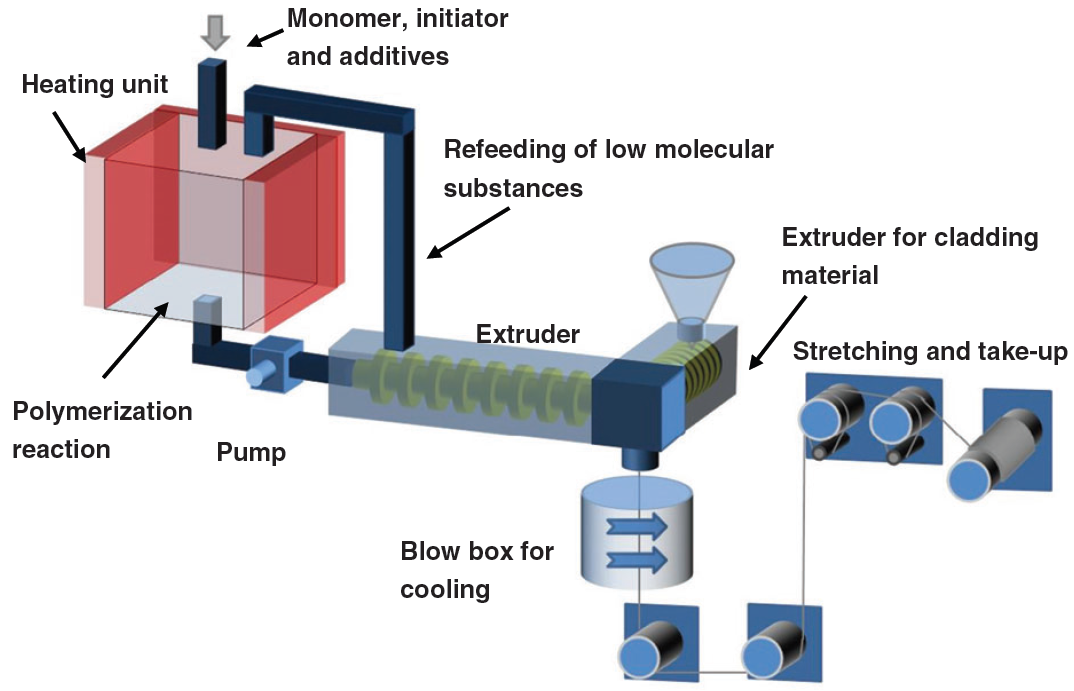
\includegraphics[height=0.25\textheight]{Bilder/Optische_Wellenleiter_Die_Polymer_Optische_Faser/Herstellung/pofsispinn.png}
                \caption[kontinuirliche Extrusion einer SI-POF \newline \url{http://www.researchgate.net/publication/265646639_An_overview_on_fabrication_methods_for_polymer_optical_fibers} S. 5 (zuletzt aufgerufen am 28.09.2015)]{kontinuirliche Extrusion einer SI-POF}
                \label{fig:pofsispinn}
            \end{center}
        \end{minipage}
    \end{center}
\end{figure}

Dieses Verfahren eignet sich ebenfalls für die Herstellung von POFs mit
\textit{Multi Step Index}. Dabei kommen jedoch mehrere Extruder zum Einsatz
(siehe \autoref{fig:pofmsispinn}), die nacheinander eine Schicht auf den Kern
auftragen und so mehrere übereinanderliegende Mäntel entstehen lassen.
\cite{pofspinn}

\begin{figure}[h]
    \begin{center}
        \begin{minipage}[t]{\textwidth}
            \begin{center}
                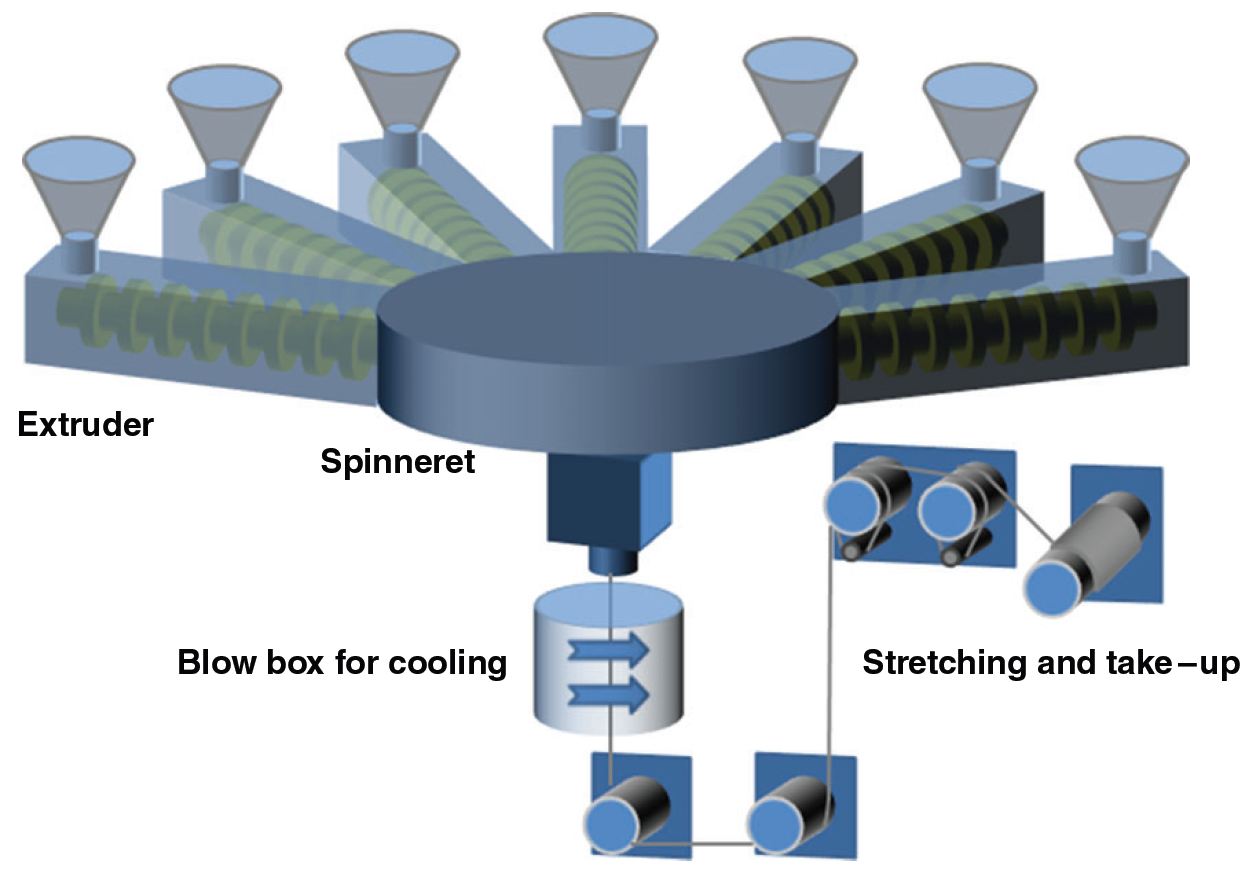
\includegraphics[height=0.25\textheight]{Bilder/Optische_Wellenleiter_Die_Polymer_Optische_Faser/Herstellung/pofmsispinn.png}
                \caption[kontinuirliche Extrusion einer SI-POF \newline \url{http://www.researchgate.net/publication/265646639_An_overview_on_fabrication_methods_for_polymer_optical_fibers} S. 5 (zuletzt aufgerufen am 28.09.2015)]{kontinuirliche Extrusion einer SI-POF}
                \label{fig:pofmsispinn}
            \end{center}
        \end{minipage}
    \end{center}
\end{figure}

\subsubsection{Herstellung einer GI-POF mittels eines modifiziertem Schmelzspinnprozesses}

Ein weiteres Herstellungsverfahren besteht in einem modifizierten
Schmelzspinnprozess der RWTH Aachen. Dieses Verfahren eignet sich für die
Herstellung von POFs mit einem Gradientenindexprofil. \autoref{fig:pofgispinn}
zeigt die nötige Produktionsanlage bestehend aus einem Einfülltrichter
(\textit{hopper}) für das granulierte Kernmaterial, einem Extruder, welcher das
Granulat erhitzt und in die Spinndüse (\textit{spinning nozzle}) drückt. Die
Spinndüse wandelt die erhitzte Kernmaterialmasse zu einem Faden um. Dieser wird
durch das Wasserbad (\textit{water quench}) gezogen. Dabei ist der
Abkühlungsvorgang für Gradientenindexprofil verantwortlich. Die Kühlungsraten
nehmen von außen nach innen ab und beinträchtigen damit die Dichte
beziehungsweise den Brechzahlenverlauf. In der letzten Einheit wird der
Polymerfaden gedehnt und aufgewickelt Die Vorteile dieses Verfahrens liegt zu
einem in der ununterbrochenen Produktion des Wellenleiters und der damit
verbundenen Wirtschaftlichkeit, da keine Unterbrechungen nötig sind, und zum
anderen in der Möglichkeit die Brechzahlen durch Variierung der Verweilzeit des
Fadens im Wasser und der Wassertemperatur zu beeinflussen.  \cite{pofspinn}

\begin{figure}[h]
    \begin{center}
        \begin{minipage}[t]{\textwidth}
            \begin{center}
                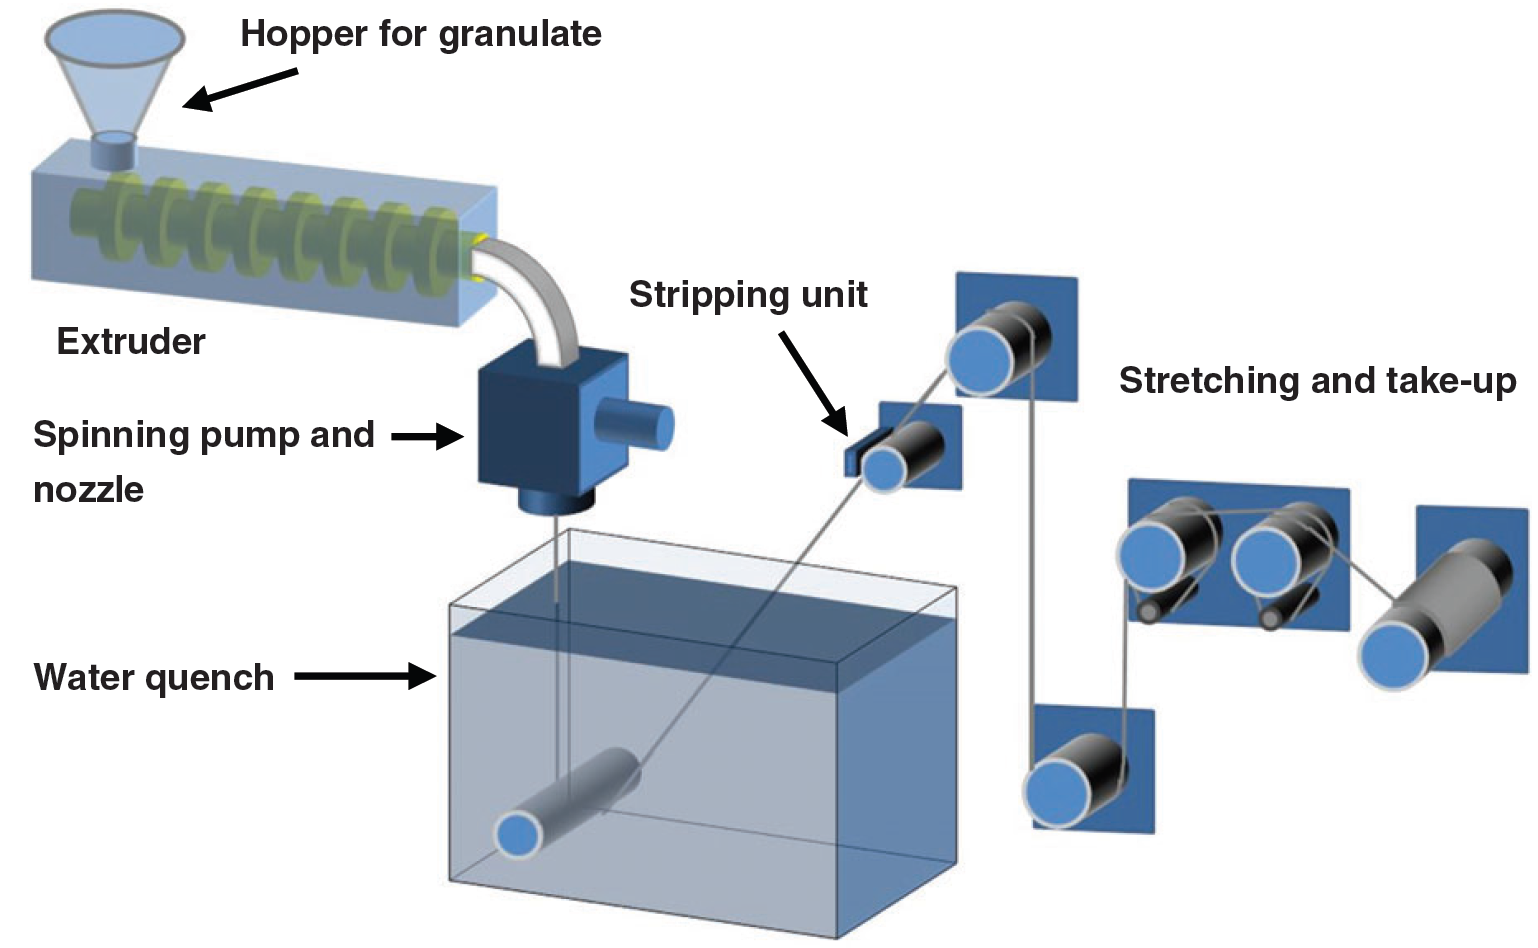
\includegraphics[height=0.25\textheight]{Bilder/Optische_Wellenleiter_Die_Polymer_Optische_Faser/Herstellung/pofgispinn.png}
                \caption[Schmelzspinnprozess zur Herstellung einer GI-POF \newline \url{http://www.researchgate.net/publication/265646639_An_overview_on_fabrication_methods_for_polymer_optical_fibers} S. 9 (zuletzt aufgerufen am 28.09.2015)]{Schmelzspinnprozess zur Herstellung einer GI-POF}
                \label{fig:pofgispinn}
            \end{center}
        \end{minipage}
    \end{center}
\end{figure}

\subsection{Vergleich zur Glasfaser}

\section{Schluss}
\label{sec:schluss}


\begin{thebibliography}{99}

\bibitem{schallplatte1}{UNI-Protokolle: Schallplatte, zuletzt aufgerufen am
01.07.2015 \newline
\url{http://www.uni-protokolle.de/Lexikon/Schallplatte.html}}

\bibitem{kassette1}{Tonaufzeichnung damals \& heute: Compact-Cassette: Ein
Renner vor allem bei Kindern, zuletzt aufgerufen am 01.07.2015 \newline
\url{http://www.tonaufzeichnung.de/medien/compactcassette}}

\bibitem{kassette2}{UNI-Protokolle: Tonband, zuletzt aufgerufen am 01.07.2015
\newline \url{http://www.uni-protokolle.de/Lexikon/Tonband.html}}

\bibitem{cd_durchbruch}{Bundesverband Musikindustrie: Musikindustrie in Zahlen,
S. 7, zuletzt aufgerufen am 01.07.2015 \newline
\url{http://www.musikindustrie.de/uploads/media/140325\_BVMI\_2013\_Jahrbuch\_ePaper\_V02.pdf}}

\bibitem{schellack}{VERBRAUCHER INITIATIVE e.V. (Bundesverband): Informationen
zu Lebensmittelzusatzstoffen, zuletzt aufgerufen am 23.07.2015 \newline
\url{http://www.zusatzstoffe-online.de/zusatzstoffe/274.e904_schellack.html}}

\bibitem{cds}{Schouhammer Immink, Kees A.: The Compact Disc Story* in Journal of
the Audio Engineering Society (Vol. 46, No. 5, 1998 May)}

\bibitem{cuz}{Roth, Klaus: CD, DVD \& Co.: Die Chemie der schillernden
Scheiben, in: Chemie in unserer Zeit (41/2007), S. 334-336}

\bibitem{cd1}{CCInfo: Compact-Disc, zuletzt aufgerufen am 03.08.2015 \newline
\url{http://www.elektronikinfo.de/audio/cd.htm}}

\bibitem{cfcd}{Didaktik der Chemie / Universität Bayreuth: Die Chemie und
Funktionsweise der CD und DVD, zuletzt aufgerufen am 07.08.2015 \newline
\url{http://daten.didaktikchemie.uni-bayreuth.de/umat/cd_dvd/cd_dvd.htm}}

\bibitem{cdp}{Asshoff, Jörg: Optische Datenspeicher - Der CD-Player \newline
\url{http://www.muenster.de/~asshoff/physik/cd/cdplayer.htm}}

\end{thebibliography}


\listoffigures


\end{document}
